\section{Random Forests}
Rassal orman (Random Forest), bir ensemble (bir araya getirme) algoritmasıdır. Hiper parametre seçimi yapmadan da iyi sonuçlar vermesinden dolayı popülerdir. Birden fazla alt ağaçlar oluşturarak overfitting'in önüne geçer. Her bir dal için Gini değişkeni hesaplanır. Alt daldaki Gini değişkeni, bir üst daldaki gini değişkeninden az ise o dal başarılıdır demektir. Yani en üstten en alta doğru gini değişkeni azalır. Hem sınıflandırma hem de regresyon problemlerini çözmek için kullanılabilir. Gözlemler bootstrap yöntemi ile , değişkenler Random subspace yöntemini kullanır. Random subspace tekniği, P adet değişkeni olan bir veri setinde, P'den daha az sayıda bir rastgele değişken seçerek her bir ağaç için, dallanmaların bu değişkenler üzerinden yapılması sağlanır. Böylece rastgelelik elde edilmiş olur. Bootstrap, benzer örnek oluşturmak için tek bir veri setini yeniden örnekleyen istatistiksel bir prosedürdür. Rastgele olacak şekilde asıl veri setinin 2/3'ü seçilir. Bootstrap veri setinde olmayan 1/3'lük kısıma "Out-of-Bag Dataset" denir. Random Forest, ensemble tekniğini kullanır. Ensemble, bir grup zayıf öğrenicinin güçlü bir öğrenici oluşturmak için bir araya gelmesidir. Ensemble, temelinde 2 yaklaşım vardır:

\begin{itemize}
    \item \textbf{Bagging:} Birçok zayıf öğrenme modelini bağımsız olarak eğitip birleştirir. Ana fikir, veri kümesinin rastgele alt küme (bootstrap) kullanılarak farklı modellerin eğitilmesi ve bu modellerin sonuçlarının birleştirilmesidir. Temel amacı varyansı azaltmaktır.
    \item \textbf{Boosting:} Zayıf öğrenme modellerini ardışık olarak eğitir ve her bir model, önceki modelin hatalarına odaklanır. Yani, hatalı sınıflandırılan örnekler üzerinde daha fazla vurgu yaparak performansı artrır. Boosting'in temel amacı bias'ı azalmaktır.
\end{itemize}

\begin{figure}[h]
    \centering
    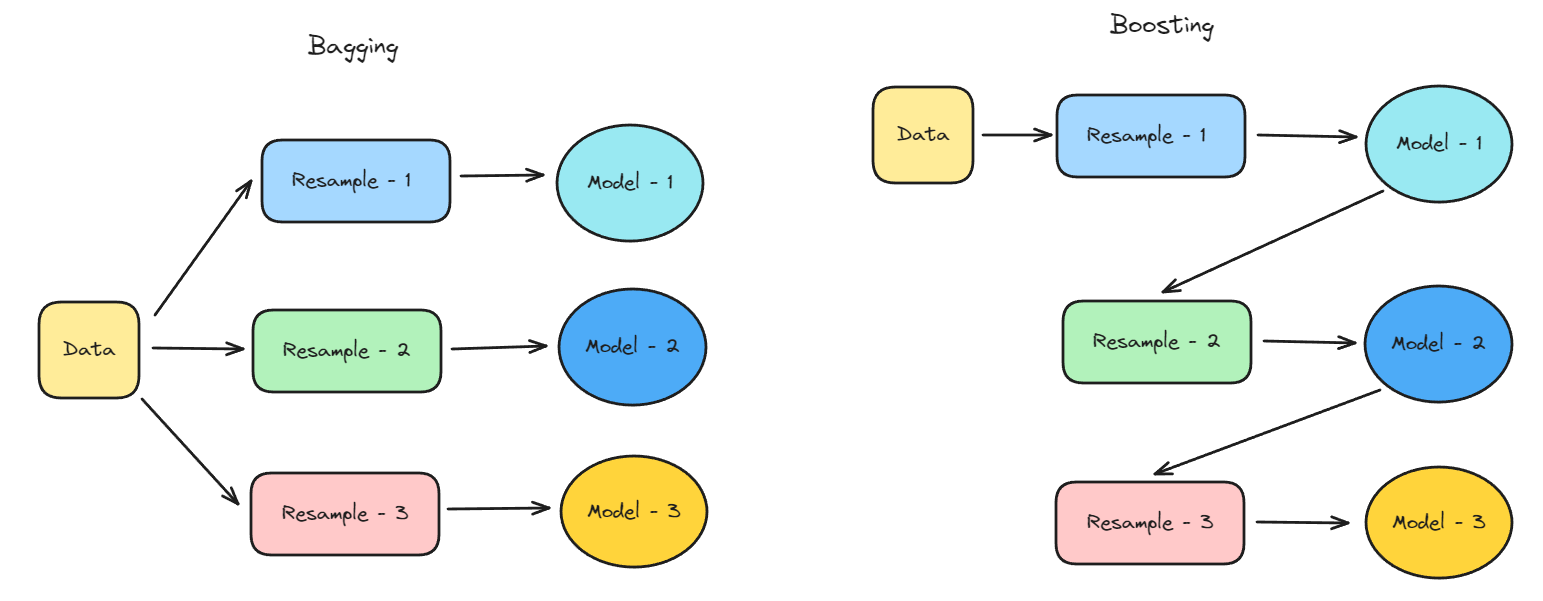
\includegraphics[width=0.7\textwidth]{images/bagging_vs_boosting.png}
    \caption{Bagging ve Boosting yöntemi.}
    \label{fig:enter-label}
\end{figure}

\subsection{Çalışma Adımları}
\begin{itemize}
    \item \textbf{Veri Toplama:} Özellikler ve hedef değişken belirlenir.
    \item \textbf{Ağaç Oluşturma (Decision Trees):} Birden fazla karar ağacı oluşturur. Her ağaç, rastgele seçilen alt örneklem verileri üzerinde kurulur. Aynı zamanda her düğümde rastgele seçilen bir alt küme özellik kullanılır. Bu, her ağacın farklı olduğu ve çeşitliliği artırdığı anlamına gelir.
    \item \textbf{Ağaçlar Arası Bağımsızlık:} Her ağac bağımsız olarak kurulur ve tahmin yapar. Bu, tek bir ağaç hatalı tahminlerde bulunursa, diğer ağaçlar da bu hatayı dengeleyebilir.
    \item \textbf{Tahmin Yapma:} Her ağacın verilen bir örnekleme için tahmin yapar. Sınıflandırma problemlerinde en çok oy alan sınıfı seçer. Regresyon problemlerinde tüm ağaçların tahminin ortalaması alınır.
    \item \textbf{Sonuç Değerlendirme:} Metrikler ile alınan sonuç değerlendirilir.
\end{itemize}

\begin{figure}[h]
    \centering
    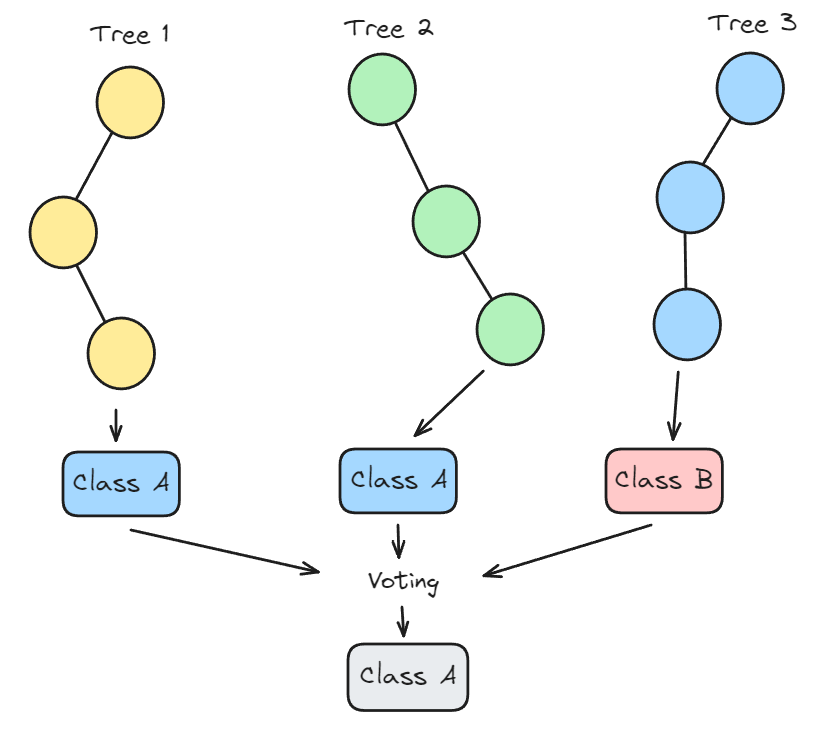
\includegraphics[width=0.7\textwidth]{images/random_forest.png}
    \caption{Rassal orman.}
    \label{fig:enter-label}
\end{figure}

\subsection{Avantajlar}
\begin{itemize}
    \item Çok kararlı bir algoritmadır.
    \item Sınıflandırma problemlerinde iyidir.
    \item Ağaçları oluşturmada veri setinin 2/3'ü kullanılır. Kalan veri performans testi ve değişken önemi için kullanılır.
    \item Her düğüm noktasında rastgele değişken seçimi yapılır. (Regression: p/3, Classification: square(p))
    \item Her bir ağaca daha önce hesaplanan hata oranları göz önüna alınarak ağırlık verilir. Çok başarısız olan ağaçların tahmini önemsenmez. Bu özellik Random Forests'i, Bagging'ten ayıran en büyük özelliktir.
    \item Eksik değerlerle başa çıkabilir. Medyan değeri kullanma ve eksik değerlerin yakınlık ağırlıklı ortalamasını hesaplama.
\end{itemize}

\subsection{Dezavantajlar}
\begin{itemize}
    \item Yorumlaması zor.
    \item Regresyon problemlerinde, sınıflandırma problemlerindeki kadar iyi bir sonuç vermez.
    \item Karmaşıklık.
    \item Tahmin üretmede yavaştır. Çünkü tahmin için tüm ağaçların aynı veri için tahmin yapıp olması gerekir.
\end{itemize}

\subsection{Hiperparametreler}
\begin{table}[h]
\centering
{\scriptsize\renewcommand{\arraystretch}{0.4}
{\resizebox*{\linewidth}{0.5\textwidth}{
\begin{tabular}{|p{3cm}|p{1cm}|p{1cm}|p{6cm}|}
\hline
Parametre & Type & Default & Açıklama \\ \hline
n\_estimators & int & 100 & Ağaç sayısını belirler. Daha fazla ağaç daha iyi performans verebilir. \\ \hline
max\_depth & int & None & Bir ağacın maksimum derinliğini belirler. Çok derin olursa overfitting'e yol açabilir. \\ \hline
min\_samples\_split & int/float & 2 & Bir düğümün bölünmeden önce kaç örnek içermesi gerektiğini belirler. Büyük olması, modelin daha basit ve daha az karmaşık olmasına neden olabilir. \\ \hline
min\_samples\_leaf & int/float & 1 & Bir yaprağın minimum örnek sayısını belirler. Yaprak düğümlerinin boyutunu kontrol eder. Küçük değer overfitting'e yol açabilir. \\ \hline
max\_features & "sqrt", "log2", None, int/float & "sqrt" & Her düğümdeki en iyi bölme özelliği seçilirken seçilen özellik sayısını sınırlar. Bu, rastgelelik ekleyerek modelin çeşitliliğini artırabilir ve aşırı uydurmayı engelleyebilir. \\ \hline
boostrap & bool & True & Veri örnekleme işleminin kullanılıp kullanılmayacağını kontrol eder. Her ağacın rastgele bir örneklemle eğitilmesini sağlar. \\ \hline

\end{tabular}
}}}
\end{table}

\newpage